\item \textbf{{[}RVHS/PRELIM/9597/2017/P1/Q2{]} }

\textbf{Missing phone number digits }

Your friend (Mary) made an oversea friend (Jenny) yesterday while
she was studying in the regional library. To remain in contact, Jenny
gave Marry her phone number and told Mary that it is also a valid
10 digits International Standard Book Number (ISBN). 

After Jenny had left, Mary accidentally punched a few holes on the
phone number while she was arranging her notes using the library\textquoteright s
hole puncher machine. It was too difficult for Mary to recover the
lost pieces of paper. So, Mary decided to look for you to recover
the missing digits instead. Below is the picture of the paper.
\noindent \begin{center}
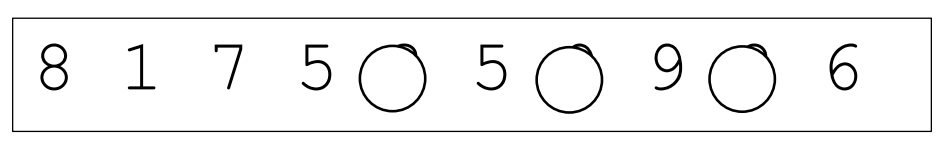
\includegraphics[width=0.5\paperwidth]{C:/Users/Admin/Desktop/Github/question_bank/LyX/static/img/9597-RHVS-2017-P1-Q1-1}
\par\end{center}

To recover the missing digits, you need to understand how ISBN-10
works. The steps to check for a valid ISBN-10 is as follow: 
\begin{enumerate}
\item[1.]  Each of the digits of the ISBN-10 is first multiplied by a number
in a sequence from 10 to 1 (Take note that the last digit of the ISBN-10
can be \textquoteleft X\textquoteright{} which holds a value of 10).
\item[2.]  All the 10 digits are then added up together. 
\item[3.]  If the sum is divisible by 11, it is a valid ISBN-10, else it is
invalid. 
\end{enumerate}
For example, to check if \textquoteleft 997150233X\textquoteright{}
is a valid ISBM-10:

\noindent %
\noindent\begin{minipage}[t]{1\columnwidth}%
\emph{Step 1 and 2}

\emph{
\begin{align*}
 & (9\times10)+(9\times9)+(7\times8)+(1\times7)+(5\times6)+(0\times5)+(2\times4)+(3\times3)+(3\times2)+(\boldsymbol{X}\times1)\\
= & (9\times10)+(9\times9)+(7\times8)+(1\times7)+(5\times6)+(0\times5)+(2\times4)+(3\times3)+(3\times2)+(\boldsymbol{10}\times1)\\
= & 297
\end{align*}
}

\emph{Step 3}

\emph{297 is a multiple of 11. Therefore, \textquoteleft 997150233X\textquoteright{}
is a valid ISBN-10. }%
\end{minipage}

\subsection*{Task 2.1}

Write a function \texttt{is\_valid\_ISBN10(isbn10)} which takes a
string \texttt{isbn10} as input and returns \texttt{True} if \texttt{isdn10}
is a valid ISBN-10 and \texttt{False} otherwise. You are to validate
the input string \texttt{isbn10} and print to terminal the issue related
to the \texttt{isbn10} string. The possible issues to be printed to
terminal includes:
\begin{itemize}
\item \texttt{ISBN-10 must only have 10 digits. }
\item \texttt{ISBN-10 can only contain numbers and the character 'X'. }
\item \texttt{'X' can only be found at the last digit of isbn10. }
\item \texttt{Wrong check digit.}
\item \texttt{Valid ISBN-10. }
\end{itemize}

\subsection*{Evidence 7 }

The program code for the function \texttt{is\_valid\_ISBN10(isbn10)}.
\hfill{}{[}6{]}

\subsection*{Task 2.2 }

Write a function \texttt{possible\_ISBN(isbn)} which takes a query
string \texttt{isbn10} as input and returns a list of possible ISBN-10.
The query string \texttt{isbn10} has 3 missing digits replaced with
a '\texttt{?}' and they can be at any positions of the query string. 

For example, 

\noindent %
\noindent\begin{minipage}[t]{1\columnwidth}%
\texttt{>\textcompwordmark >\textcompwordmark > possible\_ISBN(\textquotedbl 9971??23?X\textquotedbl ) }

\texttt{>\textcompwordmark >\textcompwordmark > {[}'997100237X',
'997102232X', '997103235X', '997104238X', '997105230X', '997106233X',
'997107236X', '997108239X', '997109231X', '997110234X', '997111237X',
'997113232X', '997114235X', '997115238X', '997116230X', '997117233X',
'997118236X', '997119239X', '997120231X', '997121234X', '997122237X',
'997124232X', '997125235X', '997126238X', '997127230X', '997128233X',
'997129236X', '997130239X', '997131231X', '997132234X', '997133237X',
'997135232X', '997136235X', '997137238X', '997138230X', '997139233X',
'997140236X', '997141239X', '997142231X', '997143234X', '997144237X',
'997146232X', '997147235X', '997148238X', '997149230X', '997150233X',
'997151236X', '997152239X', '997153231X', '997154234X', '997155237X',
'997157232X', '997158235X', '997159238X', '997160230X', '997161233X',
'997162236X', '997163239X', '997164231X', '997165234X', '997166237X',
'997168232X', '997169235X', '997170238X', '997171230X', '997172233X',
'997173236X', '997174239X', '997175231X', '997176234X', '997177237X',
'997179232X', '997180235X', '997181238X', '997182230X', '997183233X',
'997184236X', '997185239X', '997186231X', '997187234X', '997188237X',
'997190232X', '997191235X', '997192238X', '997193230X', '997194233X',
'997195236X', '997196239X', '997197231X', '997198234X', '997199237X'{]}}%
\end{minipage}

\subsection*{Evidence 8 }

The program code for the function \texttt{possible\_ISBN(isbn)}. \hfill{}{[}6{]}

\subsection*{Task 2.3}

Examine the missing numbers in the paper closely and eliminate impossible
digit choices. For example, the three missing digits cannot be \textquoteleft 1\textquoteright{}
as the three missing digits in the paper have round edges at the top.
Modify your solution in Task 2.2 and suggest these possible ISBN-10
to Mary.

\subsection*{Evidence 9 }

The screenshot of the suggested possible ISBN-10 that you will give
to Mary.\hfill{} {[}2{]}

\subsection*{Task 2.4 }

Write a menu to help other to generate possible ISBN-10. The menu
should have the following functions. 
\noindent \begin{center}
\begin{tabular}{|l|}
\hline 
\texttt{Menu}\tabularnewline
\texttt{A) Input a ISBN-10 query string}\tabularnewline
\texttt{B) Display all possible ISBN-10}\tabularnewline
\texttt{C) Quit}\tabularnewline
\hline 
\end{tabular}
\par\end{center}

You should validate user inputs and call for re-entry when an invalid
option is given. 

\subsection*{Evidence 10}

Program code for the procedure \texttt{menu()}.\hfill{} {[}6{]}